%!TEX root = pfc-memoria.tex
%!TEX encoding = UTF-8 Unicode

\chapter{Diseño de la solución}

\epigraph{``La función de un buen software es hacer que lo complejo aparente ser simple.''}{\textsc{Grady Booch} (1955--)}

En este capítulo comentamos las decisiones de diseño tomadas para la construcción de la aplicación teniendo en cuenta la ERS del \fullref{chap:analisis-requisitos}.

\section{Patrón de diseño}

Como la aplicación será una aplicación de escritorio, con su interfaz gráfica de usuario (GUI), diseñaremos el sistema de manera adecuada para dar soporte a un desarrollo rápido de la aplicación dirigida por eventos \emph{(Event-driven programming).}\index{EDP}\index{Event-driven programming@\emph{Event-driven programming}}

Se diseñará un sistema basado en el patrón Modelo-Vista-Presentador (MVP, \emph{Model-View-Presenter} en inglés)\index{MVP}\index{Modelo-Vista-Presentador}\index{Model-View-Presenter@\emph{Model-View-Presenter}}. Es un patrón parecido al conocido Modelo-Vista-Controlador (MVC, \emph{Model-View-Controller} en inglés)\index{MVC}\index{Modelo-Vista-Controlador}\index{Model-View-Controller@\emph{Model-View-Controller}}, sin embargo presenta algunas diferencias que cabe destacar (véase \autoref{fig:MVP-MVC}):

\begin{itemize}
\item En el MVP, el Controlador pasa a llamarse Presentador, y se define como un Controlador-supervisor, colocándose como hombre-en-el-medio (mitm, \emph{man-in-the-middle})\index{mitm}\index{man-in-the-middle@\emph{man-in-the-middle}} entre la Vista y el Modelo.
\item Así, el Modelo no puede interactuar con la Vista de manera directa, sino sólo a través del Presentador.
\item Esto permite mayor independencia de código y mayores oportunidades de reutilización, al ser más sencillo cambiar la Vista por otra sin afectar al Modelo, que contiene el acceso a la información y la lógica de negocio.
\end{itemize}

\begin{figure}[htbp]\centering
\begin{subfigure}[b]{0.49\textwidth}\centering
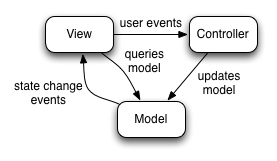
\includegraphics[width=0.85\textwidth]{MVC}
\caption{Modelo-Vista-Controlador (MVC)}
\end{subfigure}
\begin{subfigure}[b]{0.49\textwidth}\centering
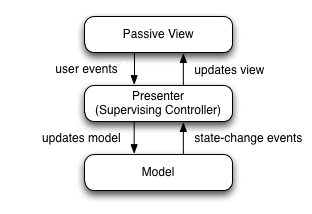
\includegraphics[width=0.94\textwidth]{MVP}
\caption{Modelo-Vista-Presentador (MVP)}
\end{subfigure}
\caption[Patrones MVC y MVP]{Patrones MVC y MVP. La principal diferencia en MVP es que el Modelo no puede interactuar con la Vista si no es a través del Presentador. \\
{\footnotesize \url{http://www.gwtproject.org/articles/testing_methodologies_using_gwt.html}}}
\label{fig:MVP-MVC}
\end{figure}

\section{Arquitectura del sistema}

La aplicación se desarrolla usando el lenguaje de programación Python~3.

En la \fullref{fig:architecture} se encuentra un resumen visual de la situación de cada componente dentro del patrón MVP y la colaboración entre ellos.

Los componentes (todos de software libre) que se reutilizan son:
\begin{description}
\item[Qt5]\index{Qt} Biblioteca de herramientas gráficas para la creación de interfaces de usuario ---con licencia de software libre--- en C++ que proporciona widgets y un framework de desarrollo de GUI compatible con la programación dirigida por eventos, soportado por las plataformas Windows, GNU/Linux y Mac~OS~X, entre otros \citep{Huang2015}. Actualmente mantenido por Digia.
\item[PyQt5] Puente \emph{(binding)} entre Python~2/3 y la biblioteca Qt5, mantenido por Riverbank Computing \citep{Summerfield2008}.
\item[QML] \emph{Qt Markup Language}\index{QML} es un motor declarativo de interfaces de usuario para Qt con sintaxis compatible con ECMAScript, integrado dentro de las versiones modernas de Qt5 \citep{web:QmlBook}.
\item[NLTK3] \emph{Natural Language Toolkit}\index{NLKT} es una biblioteca de utilidades en procesamiento de texto para Python \citep{Perkins2014}.
\item[scikit-learn] Biblioteca en Python para aprendizaje automático \citep{Pedregosa2011}.
\item[NumPy] Biblioteca en Python/C++ para el tratamiento de vectores/matrices numéricos y precisión arbitraria de manera eficiente desde Python \citep{Bressert2012}.
\end{description}

Los componentes a desarrollar son dos módulos en Python, uno para cubrir el \fullrefSRSObj{gui}, y el segundo módulo para el \fullrefSRSObj{biblioteca-nlp-ml}; y que se describen a continuación:
\begin{description}
\item[\codep{pfcsamr.gui}] Implementa el Presentador que recibe y maneja los eventos generados por el usuario al interactuar en el GUI, y canaliza las operaciones comandadas hacia el Modelo. Así mismo, monitoriza los cambios que se produzcan en el Modelo y refleja estos cambios en el GUI actualizando el estado de la pantalla. Este modelo incluye también la descripción de la interfaz en el lenguaje declarativo QML.\index{QML}
\item[\codep{pfcsamr.orchestrator}] Implementa el Modelo que actúa «orquestando» todo el proceso de análisis de sentimiento, coordinando de manera coherente los paquetes de NLTK3 y scikit-learn, y ofreciendo toda la funcionalidad de E/S.
\end{description}

Los componentes a desarrollar se indican en color verde en la \autoref{fig:architecture}, mientras el resto son componentes proporcionados por proyectos de software libre disponibles públicamente.

\begin{figure}[htbp]
\centering
\vspace{0.5cm}
\resizebox{0.75\textwidth}{!}{\input{architecture.puml.tex}}
\caption{Diagrama de arquitectura de componentes}
\label{fig:architecture}
\end{figure}

\section{Interfaz de usuario}

A continuación se muestran los bocetos de las pantallas a crear.

\subsection{Elementos comunes}

La pantalla principal es una ventana formada por 5 pestañas que guían al alumno a lo largo de las etapas de una tarea de análisis de sentimiento, y en la parte inferior una tabla de los datos obtenidos en cada etapa (\autoref{fig:gui-1-load}).

Todas las pantallas comparten los siguientes elementos:
\begin{enumerate}
\item Barra de menú, con las siguientes opciones:
\begin{enumerate}
\item \menu{File > New} (atajo de teclado: \keys{\cmd+N})\\
Pulsando esta opción se reestablece toda la configuración con los valores por defecto para iniciar una nueva sesión con un documento nuevo.
\item \menu{File > Open...} (atajo de teclado: \keys{\cmd+O})\\
Pulsando esta opción se puede abrir un fichero \path{project.yaml} del que leer el diccionario de configuración de la sesión, y se actualiza la sesión con la información leída. Véase \fullrefSRSUc{loadyaml}.
\item \menu{File > Save...} (atajo de teclado: \keys{\cmd+S})\\
Pulsando esta opción se guarda un fichero \path{project.yaml} con el diccionario de la configuración de la sesión en curso. Véase \fullrefSRSUc{saveyaml}.
\item \menu{File > Quit} (atajo de teclado: \keys{\cmd+Q})\\
Cierra la aplicación.
\end{enumerate}
\item Mitad superior con las pestañas ordenadas para guiar en el proceso: Load, Preprocess, Features, Learn y Classify, y el panel de configuración de opciones de cada etapa.
\item Mitad inferior con la tabla de datos de resultados de cada operación, en columnas y filas con controles de desplazamiento horizontal y vertical.
\item Barra de estado con tres elementos:
\begin{enumerate}
\item Texto descriptivo para mostrar qué se está haciendo o qué operación se ha terminado.
\item Barra de progreso de la operación.
\item Contador de la iteración actual de la operación en curso. Se incrementa en pasos de 32 en 32 filas para no penalizar el rendimiento con actualizaciones constantes.
\end{enumerate}
\end{enumerate}

\FloatBarrier
\newpage
\subsection{Pestaña LOAD}

La primera pestaña, \nombrebf{LOAD} sirve para cargar el fichero de entrenamiento \path{train.tsv} (\autoref{fig:gui-1-load}).

Contiene los siguientes elementos:
\begin{enumerate}
\item Botón para desplegar el selector de fichero.
\item Etiqueta de texto para visualizar la ruta al fichero.
\item Casilla de verificación para habilitar la carga parcial.
\item Selector numérico del número de primeras líneas de la carga parcial.
\item Botón de carga.
\end{enumerate}

La funcionalidad de los elementos siguen la especificación del \fullrefSRSUc{loadtraintsv}.

\begin{figure}[htbp]
\centering
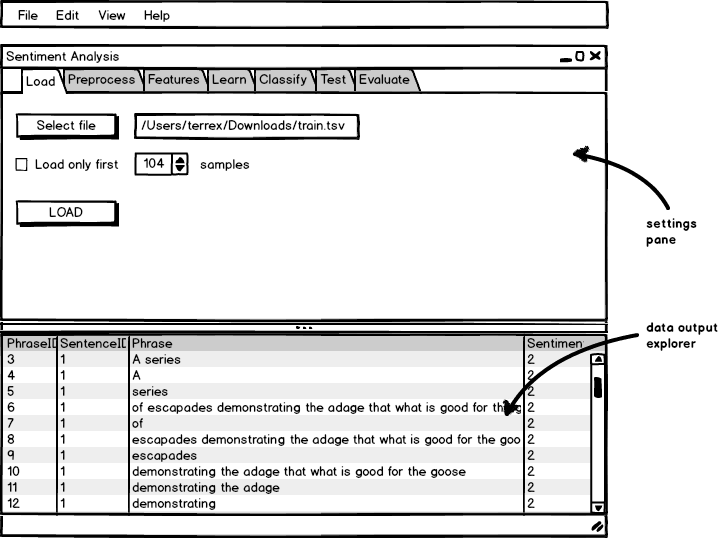
\includegraphics[width=14cm]{gui-1-load}
\caption{Wireframe de la pestaña LOAD}
\label{fig:gui-1-load}
\end{figure}

\FloatBarrier
\newpage
\subsection{Pestaña PREPROCESS}

La segunda pestaña, \nombrebf{PREPROCESS} sirve para preprocesar el texto de los documentos de entrenamiento aplicando los filtros y transformaciones indicados (\autoref{fig:gui-2-preprocess}).

Contiene los siguientes elementos:
\begin{enumerate}
\item Casilla de verificación para volver a unir las contracciones separadas.
\item Casilla de verificación para expandir las contracciones en sus palabras equivalentes sin contracción. Véase \autoref{subsec:tokenizacion}.
\item Casilla de verificación para suprimir palabras vacías (\emph{stopwords}, véase \autoref{subsec:stopwords}).
\item Casilla de verificación para habilitar el reemplazo de palabras, con una de las dos opciones excluyentes siguientes:
\begin{enumerate}
\item Radicar (\emph{stemming}, \autoref{subsec:stemming}).
\item Lematizar (\autoref{subsec:lematizacion}).
\end{enumerate}
\item Casilla de verificación para anotar la parte-de-la-oración. Véase \autoref{subsec:postagging}.
\item Botón de RUN para ejecutar la etapa.
\end{enumerate}

La funcionalidad de los elementos siguen la especificación del \fullrefSRSUc{preproc}.

\begin{figure}[htbp]
\centering
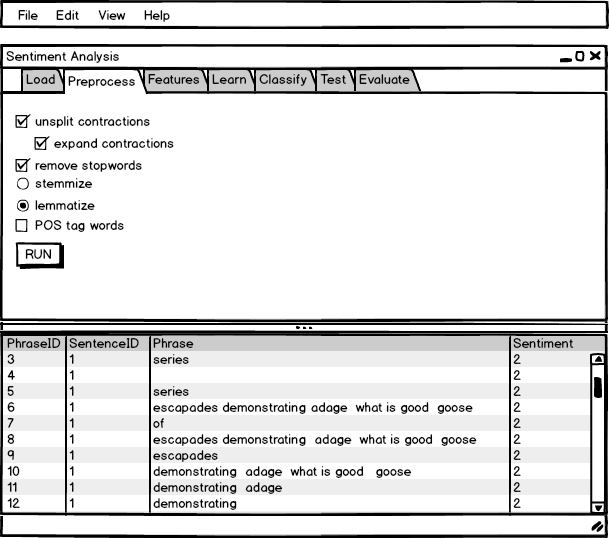
\includegraphics[width=12cm,clip=true,trim=0 0 0 38pt]{gui-2-preprocess}
\caption{Wireframe de la pestaña PREPROCESS}
\label{fig:gui-2-preprocess}
\end{figure}

\FloatBarrier
\newpage
\subsection{Pestaña FEATURES}

La tercera pestaña, \nombrebf{FEATURES} se utiliza para extraer características de los textos y vectorizar numéricamente los ejemplos del conjunto de entrenamiento (\autoref{fig:gui-3-features}).

Contiene los siguientes elementos:
\begin{enumerate}
\item Casilla de verificación y selección de $n$-gramas, en un rango de límites inferior y superior indicados en los controles de selección numérico. Véase \autoref{subsec:n-bow}.
\item Casillas de verificación para las restricciones de frecuencia documental de los $n$-gramas seleccionados, con límites mínimo y máximo, siendo las unidades el número de documentos o el porcentaje relativo.
\item Casilla de verificación para seleccionar sólo el número especificado de $n$-gramas más representativos.
\item Casilla de verificación y umbral para suprimir características con varianza despreciable (\autoref{subsec:reduccion-caracteristicas}).
\item Botón de RUN para ejecutar la etapa.
\end{enumerate}

La funcionalidad de los elementos siguen la especificación del \fullrefSRSUc{features}.

\begin{figure}[htbp]
\centering
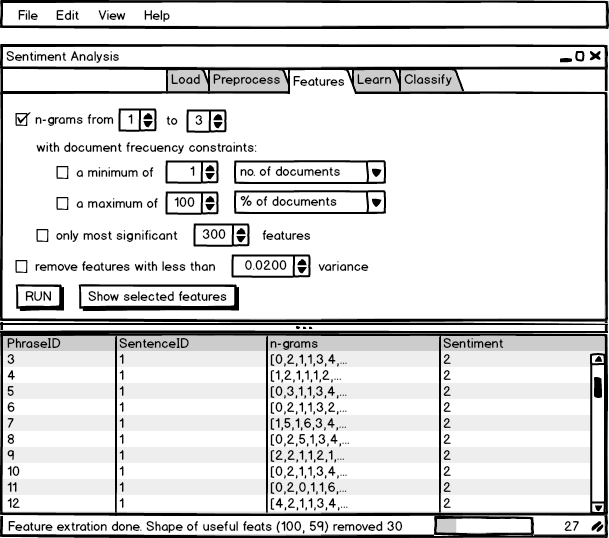
\includegraphics[width=12cm]{gui-3-features}
\caption{Wireframe de la pestaña FEATURES}
\label{fig:gui-3-features}
\end{figure}

\FloatBarrier
\newpage
\subsection{Pestaña LEARN}

La cuarta pestaña, \nombrebf{LEARN} se utiliza para extraer características de los textos y vectorizar numéricamente los ejemplos del conjunto de entrenamiento (\autoref{fig:gui-4-learn}).

Contiene los siguientes elementos:
\begin{enumerate}
\item Selección de umbral de corte para aleatorio para el subconjunto de entrenamiento y el subconjunto de autoevaluación. Si se modifica este umbral de corte, o si se activa el interruptor de «volver a dividir», se volverá a dividir aleatoriamente el conjunto completo. En otro caso, se reutilizará la división última realizada.
\item Pestañas de selección de modelo de aprendizaje. La pestaña activa es la que se utilizará para entrenar al pulsar el botón RUN, pudiendo seleccionar otra pestaña posteriormente para entrenar los demás modelos.
\begin{enumerate}
\item \codep{sklearn.MultinomialNB}. Incluye las opciones de suavizado de Laplace/Lidstone (0.00--1.00), y la opción de aprender las probabilidades a priori del conjunto de entrenamiento o bien aplicar una distribución de probabilidad a priori uniforme. Véase \fullref{subsec:MultinomialNB}.
\item \codep{sklearn.GaussianNB}. No tiene parámetros configurables (véase \fullref{subsec:GaussianNB}). 
\item \codep{sklearn.LDA}. Como opciones, contiene la selección del algoritmo de resolución, a elegir entre: a) descomposición de valores singulares, b) mínimos cuadrados, c) descomposición de autovalores. Además de la opción de número de componentes para la función (1--3) y la opción de calcular la matriz de covarianzas. Véase \fullref{subsec:lda-qda}.
\item \codep{sklearn.QDA} Incluye la opción 0.00--1.00 de ajuste del estimador de la covarianza. Por defecto: 0.04. Véase \autoref{subsec:lda-qda}.
\item \codep{sklearn.LinearSVC}. Incluye como opciones: la casilla de verificación para resolver el problema primal en lugar del dual, y el número de iteraciones máximas, por defecto 100. Véase \fullref{subsec:svm}.
\end{enumerate}
\item Botón de RUN para ejecutar la etapa. Una vez entrenado, se autoevalúa con el subconjunto de autoevaluación del umbral de corte indicado y se muestra la puntuación en la etiqueta SCORE presente al final de cada pestaña de modelo de aprendizaje.
\end{enumerate}

La funcionalidad de los elementos siguen la especificación del \fullrefSRSUc{learn}.

\begin{figure}[htbp]
\centering
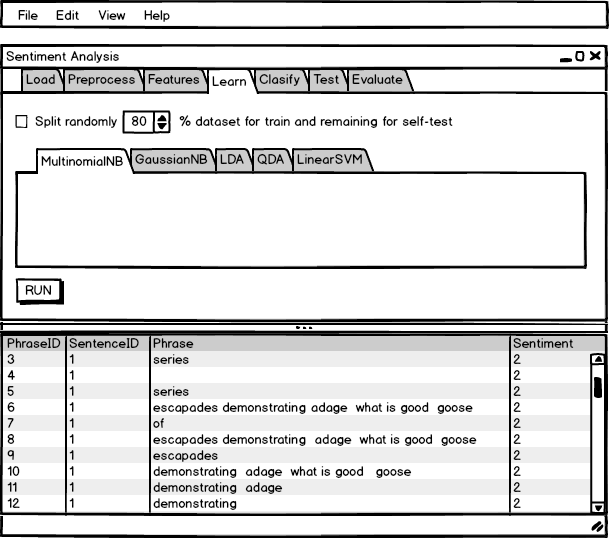
\includegraphics[width=12cm]{gui-4-learn}
\caption{Wireframe de la pestaña LEARN}
\label{fig:gui-4-learn}
\end{figure}

\FloatBarrier
\newpage
\subsection{Pestaña CLASSIFY}

La quinta y última pestaña, \nombrebf{CLASSIFY} sirve para clasificar el conjunto de prueba \path{test.tsv} (véase la \autoref{fig:gui-5-classify}).

Contiene los siguientes elementos:
\begin{enumerate}
\item Botón para desplegar el selector de fichero.
\item Etiqueta de texto para visualizar la ruta al fichero de prueba.
\item Casilla de verificación para habilitar la carga parcial, con el selector numérico del número de primeras líneas para la carga parcial.
\item Botón de carga, que realiza el \fullrefSRSUc{loadtesttsv}. Al completar, se habilita el siguiente.
\item Botón de preprocesado del conjunto de prueba en los mismos términos que el preprocesado durante el entrenamiento. Al completar, se habilita el siguiente.
\item Botón de extracción de características del conjunto de prueba en los mismos términos que la extracción y selección de características durante el entrenamiento. Al completar, se habilita el siguiente.
\item Botón de clasificación del conjunto de prueba, usando las predicciones proporcionadas por el modelo aprendido indicado en el selector de modelos. Realiza el \fullrefSRSUc{classify}.
\item Botón para exportar los resultados clasificados. Realiza el \fullrefSRSUc{savesubmissioncsv}.
\end{enumerate}

La funcionalidad de los elementos siguen la especificación de los casos de uso mencionados (\refSRSUc{loadtesttsv}, \refSRSUc{classify} y \refSRSUc{savesubmissioncsv}).

\begin{figure}[htbp]
\centering
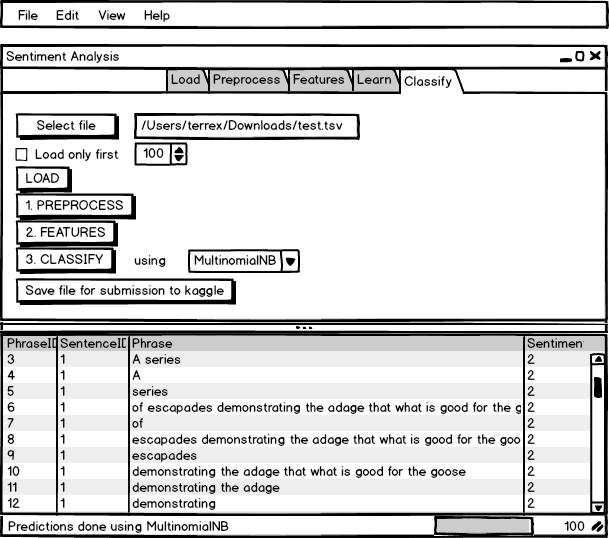
\includegraphics[width=12cm,clip=true,trim=0 0 0 38pt]{gui-5-classify}
\caption{Wireframe de la pestaña CLASSIFY}
\label{fig:gui-5-classify}
\end{figure}


\section{Clases}

A continuación se describen las clases principales necesarias. Se puede ver un resumen completo de las clases en la \fullref{fig:classes} en la página \pageref{fig:classes}.

\begin{landscape}
\begin{figure}[htbp]
\centering
\resizebox{!}{0.99\textwidth}{\input{classes.puml.tex}}
\caption{Diagrama de clases}
\label{fig:classes}
\end{figure}
\end{landscape}

\subsection{\codep{pfcsamr.gui.MainPfcsamrApp}}

\subsection{\codep{pfcsamr.orchestrator.Orchestrator}}

\subsection{\codep{pfcsamr.orchestrator.MyTableModel}}

